\chapter{Apps and their artefacts}~\label{chapter-apps-and-their-artefacts}
\julian{This chapter covers \uartefacts and \iartefacts. I'm currently drafting this chapter to try and work out what the major topics and groupings are, and then where the evidence I have fits. I'm currently inspired by \href{https://about.sourcegraph.com/blog/developer-productivity-thoughts}{A dev's thoughts on developer productivity}\citep{liu2022_a_devs_thoughts_onDeveloper_productivity} and the underlying spreadsheet of the findings is \href{https://docs.google.com/spreadsheets/d/1PcwJ6E_X6peCP1dBPADEAJXOBpnb4JY1gSGNyPSxedA/edit?usp=sharing}{here} and you should have access from your Google account if you are helping me with this thesis.}

\begin{figure}
    \centering
    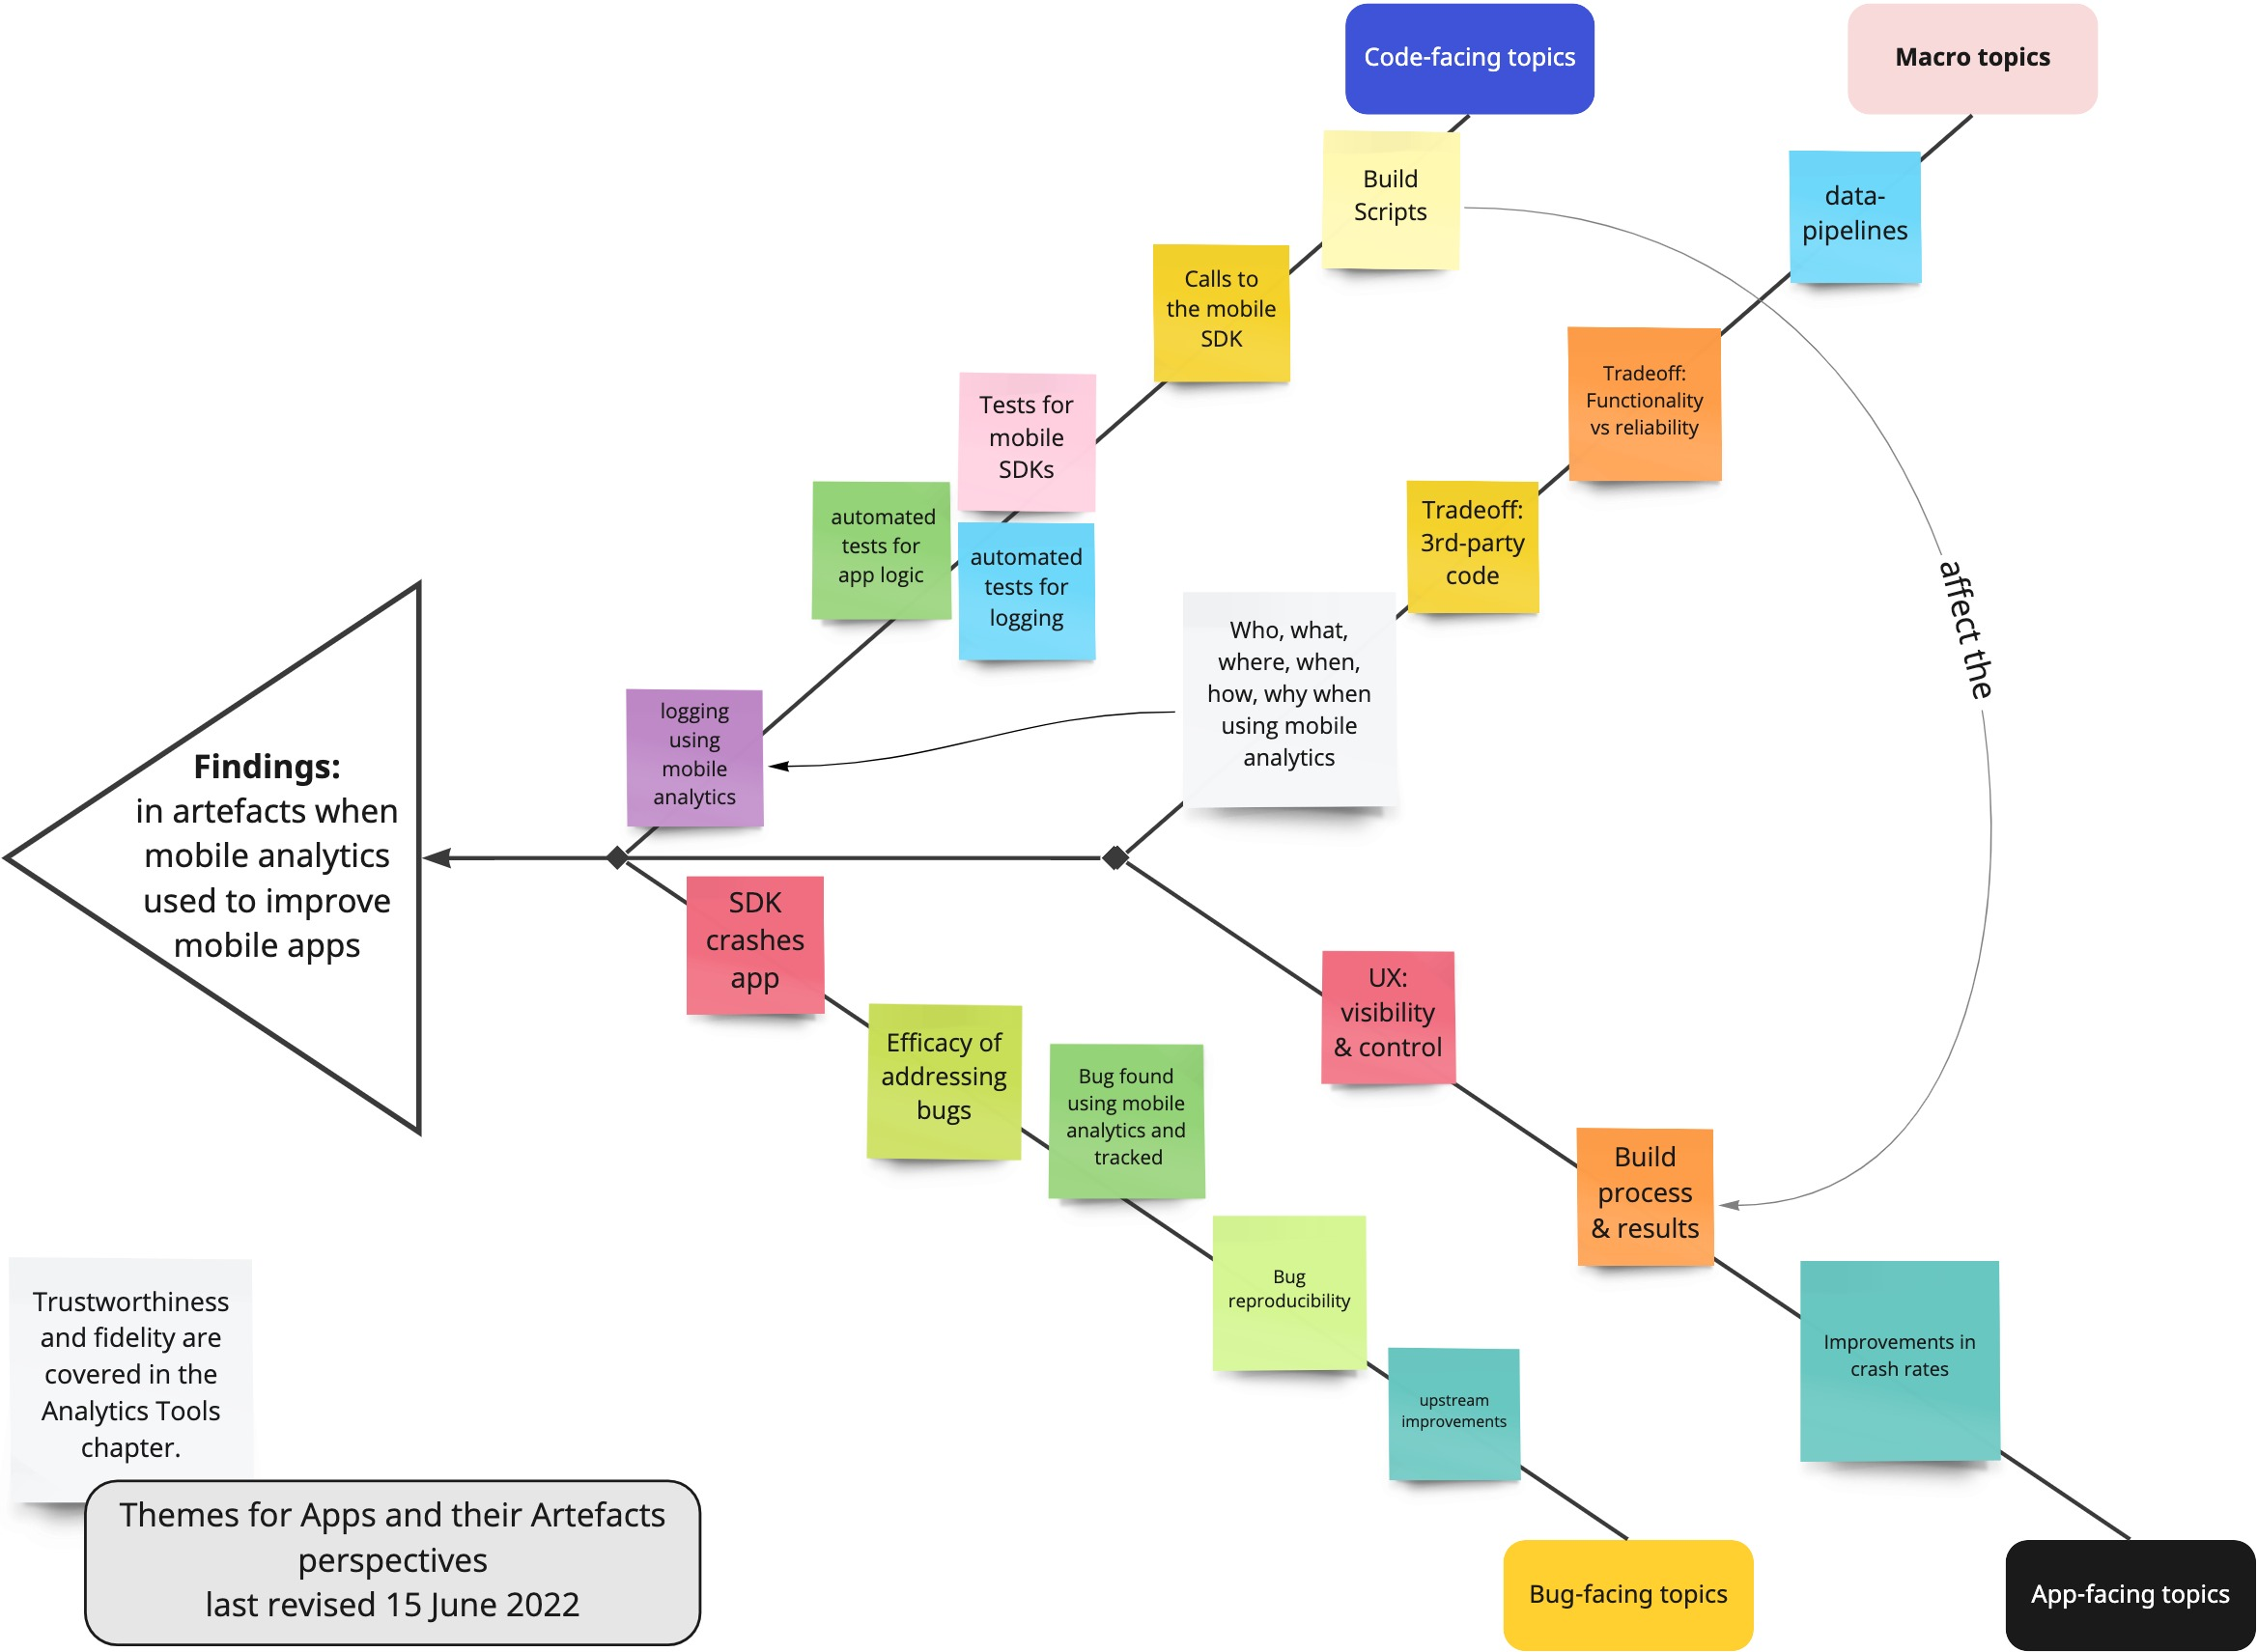
\includegraphics[width=\textwidth]{images/rough-sketches/apps-and-their-artefacts-fishbone-15-jun-2022-d.jpeg}
    \caption{Apps and their artefacts fishbone diagram\\source: \href{https://miro.com/app/board/uXjVOts6mvo=/?share_link_id=402034254193}{diagram on miro.com}}
    \label{fig:apps-and-their-artefacts-fishbone}
\end{figure}
% Note on 12-Jun-2022: Using miro's fishbone design has been helpful both in terms of me realising that I'd like a better way to illustrate the material and also to help me decide what material belongs in which chapter. Several items will be relocated from this chapter to other chapters, these are shown in the figure as free standing grey post-its. There are two links between topics, these are shown with directional arrows.

The artefacts are a product, an outcome, of what developers do as they create and maintain their mobile apps. They include the source code of the codebase which evolves on an ongoing basis for active projects, any bug-tracking/bug-management system, outputs from builds including test results, outputs from mobile analytics. 

To some extent the artefacts reflect macro (big-picture) topics including ethics, scaling, data-pipelines, engineering tradeoffs, and decisions on using third-party code. Figure \ref{fig:apps-and-their-artefacts-fishbone} illustrates the topics covered in this chapter.


\section{Code-facing topics}
\subsection{Build scripts}
App developers use and maintain build scripts to build their apps and generally the build script combines with various build tools to customise the application binary (the code that's installed on app-centric mobile devices~\footnote{There are various forms of mobile device such as 3G battery powered routers which are outside the scope of this research.}). Commonly used build variants include debug and release build targets. 

When apps include in-app mobile analytics often the build scripts are modified to specify the necessary SDK dependencies and the application's source code is modified to initialise the SDK. The documentation for Sentry's Android SDK provides a clear three step process of \textbf{Install}, \textbf{Configure}, \textbf{Verify}, so these are reproduced here~\footnote{Use permitted under their opensource license.}. Figure \ref{listing:build_gradle_for_sentry} is a typical example of how a mobile analytics dependency is added to the build file, this is Sentry's \textbf{install} step in their process.

\begin{listing}
\begin{minted}{groovy}
dependencies {
    implementation 'io.sentry:sentry-android:6.0.0'
}
\end{minted}
\caption{Example: Install Sentry \texttt{build.gradle} to an Android app's codebase\\source: \href{https://docs.sentry.io/platforms/android/}{Android Sentry Documentation}}
\label{listing:build_gradle_for_sentry}
\end{listing}

The \textbf{configuration} step requires a setting that is uniquely allocated by Sentry for this app when the developers use Sentry's online service. Listing \ref{listing:android_manifest_xml_for_sentry} shows the syntax of the configuration; the developers would need to obtain the unique dsn (data source name) to use for their app and use that value in place of the example value.

\begin{listing}
\begin{minted}{xml}
<application>
  <meta-data android:name="io.sentry.dsn"\\
  android:value="https://examplePublicKey@o0.ingest.sentry.io/0" />
</application>
\end{minted}
\caption{Example: Configure Sentry for that Android app\\source: \href{https://docs.sentry.io/platforms/android/}{Android Sentry Documentation}}
\label{listing:android_manifest_xml_for_sentry}
\end{listing}

\textbf{Verification} is not strictly part of the build scripts as it's part of the app, nonetheless it's included here since it is closely connected to the previous steps.

The code snippet in Listing \ref{listing:android_activity_to_verify_sentry_works_in_app} sends details of a caught exception to Sentry's service each time the code is run. Running this code (by using the app) helps \textbf{verify} the installation and configuration steps have been completed adequately. Note: this code would generally be removed from the app once the verification has been completed successfully, developers would effectively replace it with custom code for any additional reporting not already provided automatically by the SDK. % https://docs.sentry.io/platforms/android/usage/  https://docs.sentry.io/platforms/android/enriching-events/breadcrumbs/  https://docs.sentry.io/platforms/android/configuration/integrations/okhttp/

During the period of this research, the SDKs have continued to evolve and tend to offer developers a greater range of information and also they tend to automated more of the underlying data collection, for example the Sentry 3.1.0 Android Gradle plugin automatically instruments the OkHttp library if it's part of the app~\footnote{\url{https://docs.sentry.io/platforms/android/configuration/integrations/okhttp/}}.


\begin{listing}
\begin{minted}{kotlin}
import androidx.appcompat.app.AppCompatActivity
import android.os.Bundle
import io.sentry.Sentry

class MyActivity : AppCompatActivity() {
  override fun onCreate(savedInstanceState: Bundle?) {
    super.onCreate(savedInstanceState)
    try {
      throw Exception("This is a test.")
    } catch (e: Exception) {
      Sentry.captureException(e)
    }
  }
}
\end{minted}
\caption{Example: writing code to verify the install and configuration of the Android app\\ source: \href{https://docs.sentry.io/platforms/android/}{Android Sentry Documentation}}
\label{listing:android_activity_to_verify_sentry_works_in_app}
\end{listing}

The majority of the other SDKs used in the case studies offer equivalent installation, configuration, and verification steps and include developer-oriented documentation of these steps; note: they may use other terms to describe these steps.

\textbf{Build scripts partly encapsulate the build process}.  
At one extreme build scripts may fully automate multiple steps to the point of releasing a new version of an app in the app store, at the other extreme many of the steps may be manual and performed unsystematically by the development team. Of course many projects are somewhere between these two extremes. In one of the case studies a mistake in a manual step meant the new release of the Pocket Code did not include the correct information and stopped the in-app crash analytics from being reported. The Crashlytics SDK on Android needed two distinct keys, an API Key and a secret key~\footnote{StackOverflow has a good example of how a build script obtains these values from the environment \url{https://stackoverflow.com/q/46814593/340175}~\citep{scott2017_android_app_crash_noclassdeffounderror_on_samsung_lollipop_devices}. The relevant documentation is no longer available, it was at \url{https://docs.fabric.io/android/fabric/settings/working-in-teams.html} according to \url{https://stackoverflow.com/a/40667490/340175}}, and presumably at least one of these was either missing completely or incorrect for that build.
% https://stackoverflow.com/questions/31596792/how-to-get-test-and-production-values-for-fabric-crashlytics 
% See also https://www.instabug.com/crashlytics-alternative 
% and a nice set of examples of how to integrate various SDKs including AppSee and Crashlytics in Ruby code https://github.com/HipByte/motion-fabric 

As an aside, in Grey Data, there is an excellent example not only of configuring the API Secret Key using the runtime environment (the method used by the Catrobat project) but of an adverse side-effect of changing the build target to a newer release of Android where the app then started to crash frequently on some Samsung device models~\citep{scott2017_android_app_crash_noclassdeffounderror_on_samsung_lollipop_devices}. 


\subsection{Calls to the Mobile Analytics SDK}

\begin{itemize}
    \item Commercial project: extensive use of Microsoft App Center to record caught exceptions, in particular.
    \item Moonpig: extensive use of Firebase Analytics to record breadcrumb information to help determine and understand what led to undesirable events.
    \item 57 opensource Android apps:\pending{TBD how much to write up here vs. reference in my jointly authored paper \citep{harty2021_logging_practices_with_mobile_analytics}.} 
\end{itemize}


\subsection{Use of automated tests for the app}
Automated tests can dovetail with using mobile analytics to improve the reliability of mobile apps. For example, they can be used to demonstrate the reproducibility of crashes identified through mobile analytics. In the commercial case study this is what we did for various crashes reported via Android Vitals. For one of these an equivalent example has been released as an opensource project at \url{https://github.com/julianharty/KotlinNPE} which tests the fix. This project is partnered by another opensource project \url{https://github.com/julianharty/AutomatedTestingWithKotlin} as we wanted to find a way to run tests directly in a Java Virtual Machine (JVM) without needing the overhead of the Android runtime. When automated tests need the Android runtime the build process and the runtime environment become much more complicated and the elapsed runtime for the tests can take several orders of magnitude more time.

Use of automated tests for bug reproduction/bug fixes was patchy in all of the development teams in the case studies. \emph{I.e.} they all chose to `fix' at least some crashes directly without the support of automated tests. Their success rates of writing these fixes varied. For example the Kiwix developers were able to fix various NullPointerExceptions directly in the application's source code whereas they were not able to fix the crashes in the custom downloader code. 

Moonpig's development team chose to write automated tests where they believed they would be helpful, for some of the failures they believed they had sufficiently detailed sources of information to apply some fixes directly to the codebase, in part through their extensive use of Firebase Analytics for in-app logging and usage monitoring.

% COULD_DO if it'd be useful - review the fixes applied after the PocketCode hackathon to see how many included automated tests. Then write up the results here.


\subsection{Tests for mobile analytics SDKs}
Several types of tests have been found for mobile analytics SDKs, the first type are tests developers implement to \textit{check the plumbing works i.e.} that the SDK has been integrated and configured adequately for a basic confidence test. The second type are written to check the SDK at a unit or module level.

\textbf{Support in the SDK}: 
All of the in-app crash reporting SDKs encountered during the research included confidence tests (verifying the SDK has been configured adequately). The app-centric case studies might have used these verification tests when they enabled their mobile analytics SDKs, however as noted earlier these verification tests are unlikely to be long-term additions to the app's codebase and no evidence is available on whether they were used or not. 

\textbf{Did the app-centric case studies have crash reporting tests?} 
The Catrobat project included automated unit tests for crash reporting~\footnote{The source code for the tests is available online \url{https://github.com/Catrobat/Catroid/pull/2419/files} and the pertinent code review discussions are available online \url{https://github.com/Catrobat/Catroid/pull/2371}.} until the project removed Firebase Analytics from the project several months after the core case study~\footnote{Pull request that removed the tests \url{https://github.com/Catrobat/Catroid/pull/3832}.}. Kiwix does not use in-app mobile analytics so does not have any tests for them either. 

Automated tests for the opensource SDKs used in the app-centric case studies are available on github.com: Amplitude Android~\footnote{\url{https://github.com/amplitude/Amplitude-Android/search?q=test}}, Segment.io's Android SDK~\footnote{ \url{https://github.com/segmentio/analytics-android/search?q=test}}, Sentry's Android SDK~\footnote{\url{https://github.com/getsentry/sentry-java/search?q=test}} and React Native SDK~\footnote{\url{https://github.com/getsentry/sentry-react-native/search?q=test}}, and Firebase's Android SDK~\footnote{\url{https://github.com/firebase/firebase-android-sdk/search?q=test}}, amongst others. 

While these SDKs have various automated unit tests, end-to-end tests for the SDKs are harder to find. Segment provides an End to End test  \href{https://github.com/segmentio/analytics-android/blob/master/analytics-samples/analytics-sample/src/androidTest/java/com/segment/analytics/E2ETest.java}{E2ETest.java}~\footnote{They also provide a standalone command-line test tool \url{https://github.com/segmentio/library-e2e-tester}.}, and clearly describe why they have chosen to test their service in production~\citep{segment2018_we_test_in_production_you_should_too}.  

\subsection{Automated tests for logging}
As part of this research I co-wrote various small software projects to provide automated tests of local logging by Android apps~\citep{android_crash_dummy, android_log_assert}; these have been released under permissive opensource licenses. While logging is rarely a source of crashes in mobile apps it's often used to a) by the platform and/or the logging SDK record the actual crash and associated stack trace, and b) by the app developers to record information to help the app developers diagnose possible reasons for the crash~\footnote{As an aside, Google developers worked with app developers to add logging to help diagnose crashes for some older Android devices \url{https://github.com/google/filament/issues/2418}.}. 
% Note PostHog uses a ShadowLog in their tests of logging https://github.com/PostHog/posthog-android/blob/master/posthog/src/test/java/com/posthog/android/LoggerTest.java

\subsection{Mobile analytics for remote logging}
Some app developers also chose to use mobile analytics for logging, for example in 107 opensource Android projects available on github.com~\citep{harty2021_logging_practices_with_mobile_analytics}. Mobile Analytics SDKs tend to use a network connection to transmit information from the end-user's device to central servers~\footnote{I'm not aware of any exceptions however other transfer mechanisms are possible such as using memory cards or memory sticks.}. As an aside, it should be practical to write automated tests for mobile analytics SDKs to check the data the SDK emits. Doing so is outside the scope of this research and a possible topic for future research. % I have looked at PostHog's code which is actually based heavily on a fork of Segment's opensource code so I then also looked at some of Segment's Android code. I didn't find any code that actually checks the output or the transmission aspects. Note: https://segment.com/docs/connections/sources/catalog/libraries/mobile/android/ uses Square's Tape opensource library to persist event data. This might be something to explore adding memory-card/stick transfer to.

Logging, network IO, and mobile analytics combined in the industrial case study where a high crash rate in a new release was caused by a flawed implementation to increase the logging of network IO through the OkHttp library used by the Android app. 

\section{Bug-facing topics}

\begin{itemize}
    \itemsep0em 
    \item SDK can cause the app to crash e.g. \href{https://github.com/segmentio/analytics-android/issues/732}{Crash during Google Pre-launch report \#732}.
    \item Some developers choose to record bugs for failures reported via mobile analytics.
    \item Bug reproducibility, including the use of automated tests.
    \item The efficacy of addressing bugs.
    \item Obviating some bugs by replacing Java code with Kotlin (Upstream improvements).
\end{itemize}


\section{Macro topics}\pending{13-Jun-2022 This topic may move to the Process chapter, either partly or completely. If so, the effects on the artefacts (would still belong here). TBD when I've revisited that chapter.}
Macro-topics touch on multiple aspects of developing mobile apps. This research identified the following groupings of macro-topics:

\begin{itemize}
    \item Three of these have a common trait of \textbf{tradeoffs} developers face, in ethics, in the use of third-party code, and in functionality.
    \item Two have a common trait of \textbf{scaling}: scaling use of mobile analytics by developers and within their engineering microcosm.
    \item Two cover the trustworthiness and fidelity of the mobile analytics as reflected in the artefacts.\pending{I have an inkling this material is better placed elsewhere in my thesis than this chapter. TBD.} 
\end{itemize}

\subsection{Tradeoffs}
At least three types of tradeoffs were evident in the artefacts: 1) the effects of ethical decisions by the project team\pending{Discuss the process of the decision-making in the Process chapter, not here, then cross-reference to that material here.}, 2) downgrading functionality to obtain reliability, and 3) use of third-party vs locally developed functionality. 

\textbf{Ethics}\pending{These 2 paragraphs will be relocated to the Process chapter soon.}: 
Several of the development teams had to make explicit decisions whether to use mobile analytics and if so which one they would use. The Kiwix project team chose explicitly to exclude mobile analytics from their apps to reduce the potential for end users to be tracked and potentially imprisoned through their use of the app and Wikipedia content in particular~\footnote{The Kiwix project was developed to provide offline access to all of Wikipedia, it was then extended to support and provide lots of other content and material, nonetheless Wikipedia content is the one most likely to put end users at risk in some jurisdictions.} The Kiwix team did decide to use the platform-provided analytics from Google Play Console on the grounds that if the end-user had a) installed the Kiwix app from Google Play and b) had enabled (or at least not disabled) Google's collection of usage and performance data from their phones then the users were not being compromised by the devs using the analytics generated from the data those phones and tablets had provided.

The Catrobat team started by adding Fabric Crashlytics into their Pocket Code Android app several years before becoming a case study for this research. After seeing the results of applying the techniques from this research they choose to add Crashlytics to their iOS Pocket Code app and were also planning to use Firebase Analytics to record more granular usage data to both the Android and iOS apps. However, as a side-effect of migrating from the Fabric Analysis to Firebase Analysis - using the same client side SDK release they discovered they started receiving demographic data in tandem to the reliability analytics. Google then set a deadline where developers would need to replace the Fabric client side SDK with a similar one from Firebase to continue receiving any of the reports. The Catrobat team decided to stop using Crashlytics entirely rather than having demographics meta data collected by these SDKs in their apps. The Catrobat team had no objections to continuing to use the platform-provided analytics.

\textbf{Impact of ethical decision to remove mobile analytics}: The Catrobat project team chose explicitly to remove support for Crashlytics in the Pocket Code app when Google's deadline for migrating to Firebase Crashlytics expired. At the time, the project team discussed whether to keep Google Analytics support in the Pocket Code app. Pull Request 
\href{https://github.com/Catrobat/Catroid/pull/3832}{3832} in the Pocket Code repository provides a written record of the changes made to the codebase and the discussion.

\textbf{Reliability trumps enhanced functionality}: 
The core Kiwix Android app included a custom file downloader that downloaded material such as Wikipedia in German for offline use. This downloader kept track of partial downloads and also allowed end users to control when to allow the downloads and when to pause or stop them. This functionality was designed to help users often in areas with intermittent, controlled, and sometimes expensive connectivity to increase their chances of being able to download the content within their budget. To provide some concrete examples in some parts of the world users would download content that took several entire \emph{days} even if the connection didn't fail, and the cost of the connection was metered and capped to 1GB of data.

However, the code for the downloader had various bugs and flaws including several that caused the app to crash. These crashes meant the app had an excessively high crash rate in the Google Play App Store. The then lead developer for the Android codebase had not been able to tame the high crash rate. A consultant was hired who had worked on multiple other Android projects and codebases. This consultant proposed scrapping the custom downloader and replacing it with standard Android functionality provided by Google as part of the Android SDK. This proposal was accepted and implemented\pending{Add details of the release and commits} and it had the desired effect of reducing the crash rate of the core Kiwix Android app by about a third\pending{check details and revise accordingly}. So far, so good.

However the standard Android downloader didn't provide equivalent facilities to continue partial downloads, or to pause and resume downloads, nor did it provide progress tracking information. Furthermore as the project team had chosen not to incorporate in-app mobile analytics the project team cannot easily determine the effects of these changes \emph{on the end users}. Bugs continue to surface occasionally on the project's GitHub site~\footnote{\textit{e.g.} \url{https://github.com/kiwix/kiwix-android/issues/2845}.} and users sometimes complain in reviews submitted to Google Play. Here are four examples extracted from the developer's view of Google Play:

\begin{itemize}
    \itemsep0em
    \item ``\textit{Wikipedia nopic without images works again in version 11.18 with search function.! Top Unfortunately, now in March 21 again problems with wikipedia text with 14.2 gb. After 3/4 of the download the process breaks off every time! Too bad. Wikis with smaller amounts of data can be downloaded without any problems. Handling of the app very well.}'', Mar 22, 2021 % https://play.google.com/console/u/0/developers/9116215767541857492/app/4975184706939091905/user-feedback/review-details?reviewId=gp%3AAOqpTOGjPB5Em_o1TfLCzltkR7jvVhdVJAvBZlj9Y0-5i9FOcDaJ4Yjh1yqIHV5-qo-9HkbvGJSAHweXJOQodfo&corpus=PUBLIC_REVIEWS
    \item ``\textit{Download started and it could never finish}'', Mar 25, 2021 % https://play.google.com/console/u/0/developers/9116215767541857492/app/4975184706939091905/user-feedback/review-details?reviewId=gp%3AAOqpTOErPflFJDpyqiz4m4CJW3IPjYoXKGrO0SLZ4L94DwUPj662lAWuS0MOWAXfANZ2D6Vf--EkJLe1RPIeSqk&corpus=PUBLIC_REVIEWS
    \item ``\textit{Seems that library download is b0rken atm?}'', Oct 7, 2021 % https://play.google.com/console/u/0/developers/9116215767541857492/app/4975184706939091905/user-feedback/review-details?reviewId=gp%3AAOqpTOGVOb-MNO3ehakCJsUi7Ur-R_6QJkdnWzFDl7xh6KA28ZUATGKmBO7JzDTgPvULR0UhivkWMp2B0d83qpA&corpus=PUBLIC_REVIEWS
    \item ``\textit{Cant continue interrupted download}'', Oct 15, 2021 % https://play.google.com/console/u/0/developers/9116215767541857492/app/4975184706939091905/user-feedback/review-details?reviewId=gp%3AAOqpTOFxVKQVzPIrgcWHmCX8QnQXaqVkI8JFVwBzLYiDHJrdBbokV8SBDfRRjYltEqBp8lsLVTNFlix3fzFMHYA&corpus=PUBLIC_REVIEWS
\end{itemize}

And another review asks for the download manager that, ironically, used to exist (presumably without realising the app used to have one): ``\textit{edit: still there is no download manager. It is not possible to download the large files. Despite 100 megabits per second, I did not manage to load the large Wikipedia with images. The app itself is very good. Only the download of the huge files always breaks off. I load via PC. A download manager would not be bad.}'', Mar 12, 2021 % https://play.google.com/console/u/0/developers/9116215767541857492/app/4975184706939091905/user-feedback/review-details?reviewId=gp%3AAOqpTOEH9rOv2WWhAUTEChRwgT1Mrq5rYxEp9cQzrqjGDg6aeOccjVgxJeNFU_syr1wNPh9UMw71FKfM13iNy8k&corpus=PUBLIC_REVIEWS 

\textbf{Third-party code}: 
The third tradeoff is between third-party and locally developed code which generalises the second tradeoff found in the research (of trading functionality for reliability). As a concrete example, the WebView component is ubiquitous on Android and found in many Android apps including several of those in the case study\pending{Is it worth the investment to find out how many of the apps use the Android WebView?}. 

% Google's overview on the WebView component is available at https://developer.android.com/guide/webapps and https://developer.android.com/guide/webapps/webview-privacy discusses crash reporting and other data collection topics pertaining to apps using WebViews.

As projects, including the Kiwix team, discovered crashes can be reported in Android Vitals for the WebView component. These adversely affect the app's reliability as measured by Android Vitals. While the app developers can fix at least some of the causes of third-party components, including the WebView component, others may be beyond their direct control.

In March 2021, major apps including apps from the Amazon, BBC, Facebook, Google, Microsoft, etc. failed in use by a release of the WebView component~\citep{peters2021_google_fixes_issue_causing_android_apps_to_crash_etc_webview, bbcnews2021_google_fixes_crashing_android_app_issues, bbc_iplayer_app_april_2021_webview_information}. and Samsung's bland observation % https://www.samsung.com/ph/support/mobile-devices/google-webview-issue/ 
All their respective app developers relied on a third-party software component developed and maintained by Google as part of Android. Furthermore, app developers who have incorporated the WebView into their app sometimes introduced bugs in their use of the WebView. Across a population of 146 opensource Android apps 124 WebView related bugs were found and the root causes analysed~\citep[pp. 704 - 706]{hu2018_a_tale_of_two_cities_how_webview_introduces_bugs_to_android_applications}. Of these bugs, 15 introduced crashes~\citep[p. 706]{hu2018_a_tale_of_two_cities_how_webview_introduces_bugs_to_android_applications}.

As Google Android notes online \url{https://developer.android.com/guide/webapps} there are various alternatives to using a WebView. They don't mention either a) developers developing their own user interface, or b) other third-party alternatives to their WebView (\emph{e.g.} \href{https://mozilla.github.io/geckoview/}{Mozilla's GeckoView}). 
% https://stackoverflow.com/questions/35559467/webview-alternatives (the answer is too dated to include in my thesis). and https://www.i-programmer.info/news/193-android/12900-the-geckoview-alternative-to-webview.html 
% https://android.gadgethacks.com/how-to/ditch-googles-webview-switch-androids-system-browser-bromite-0384227/ 

There is no silver bullet for developers in terms of choosing whether to write their own code or use third-party code. Tradeoff 2 enabled the Kiwix team to improve the reliability at the cost of losing functionality; tradeoff 3 allows developers to short-circuit the work of developing their own functionality at the risk of being unable to address some of the failures and problems related to using those third-party components\pending{Describe the artefacts}.

\subsection{Scaling}
\textbf{Developers' access to, and use of, mobile analytics services}: 
In hindsight it may be blindingly obvious that in order to use mobile analytics one first needs access to the mobile analytics service and then to gain the habits and understanding to actually use what's been made available. And yet, in the majority of the case studies only a minority of the team leaders actually provided access to the majority of their team members. Examples of these case studies include LocalHalo where the CTO appeared to be the only developer with access to Sentry; in the Kiwix Android team where lead developers were the majority of those who had direct access to Android Vitals and similarly for the Catrobat project access tended to be for senior developers who were long-time team members\footnote{Note: hard data was hard to obtain given the nature of the access granted to the researcher and discussions with the projects seldom led to the data being made available.}.

In the commercial project there were challenges in determining who granted access and subsequently developers had to obtain prior approval from their manager before requesting access to mobile analytics, and new team members were not necessarily even aware of the mobile analytics services so couldn't begin to request access. 

The clear counter example was Moonpig where the development team members were routinely provided access to the mobile analytics as part of joining the development team. Furthermore the developers rotated on-duty to actively monitor the mobile analytics to find and respond to any anomalies; therefore they were encouraged to learn how to use, understand, and act on the reports in the mobile analytics services.

\textbf{System integration of mobile analytics outputs}: 
The commercial project was and is part of a much larger engineering organisation with thousands of staff members. The engineering organisation required integration of all the mobile analytics services into their data lake through data-pipelines~\footnote{A useful overview of data-pipelines from three industry case studies describes various challenges and opportunities those companies experienced~\citep{munappy2020_data_pipeline_management_in_practice_challenges_and_opportunities}.} Several of the enterprise-scale mobile analytics services, including Google Analytics 360 and Microsoft's App Center, provide high-volume exports using their respective proprietary cloud storage service. Microsoft App Center also provides an openAPI that can be used for REST queries interactively \url{https://openapi.appcenter.ms/} and/or programmatically (documented online at \url{https://docs.microsoft.com/en-us/appcenter/api-docs/}). This was used on an \emph{ad-hoc} basis during the case-study before the data-pipeline was fully established and worked adequately for the \emph{ad-hoc} work.  
% https://docs.microsoft.com/en-us/appcenter/diagnostics/using-the-diagnostics-api 

Various of the mobile analytics services provided API integration, these are covered in the \href{chapter-tools-and-their-artefacts}{Tools and their artefacts} chapter.\pending{Provide a more elegant link.}

The Google and Microsoft storage integration requires both authorisation and paying for by the organisation. In turn this meant a development team needs to get approval to access and use these services, and the approval may be time-consuming even if senior management has dictated the project will integrate and use these services as a side-effect of corporate processes and working practices. An entirely separate team may be responsible for the `plumbing' in of the project's data from the mobile analytics service where the development team needs to request the necessary work and then wait until that work has been approved, scheduled, and then attempted. As Twitter engineers noted plumbing is a key activity~\citep[page 6]{lin2013_scaling_big_data_mining_infrastructure_the_twitter_experience} 


\section{App-facing topics}

\begin{itemize}
    \itemsep0em
    \item Improvements in crash rates.
    \item Build scripts can affect the behaviour of the app.
    \item User Experience of apps with in-app analytics (visibility and control aspects).
\end{itemize}

\subsection{Improvements in crash rates}
For both Catrobat and Kiwix the hackathon and the post-hackathon bug fixes were highly effective in terms of cumulatively reducing the crash rate over several subsequent releases. % TODO Check whether the releases were contiguous.
The Catrobat case study replicated the improvements seen in the Kiwix case study and also the efficacy of using a hackathon as an immediate intervention. TODO discuss limitations of hackathons and forward link to the section on the useful half-life of hackathons. 


For Pocket Code, the improvements in the stability of the app were particularly encouraging as the project had already implemented many of `good' development practices.


\textbf{TODO include the other case studies.}

\section{Discussion}\label{apps-and-artefacts-discussion-section}
Much of a developer's focus, perhaps unsurprisingly, is working with code and modifying code to achieve various objectives. An industry-focused article by Beyang Liu discusses the author's thoughts on developer productivity and introduces a term `\textbf{developer hertz}' as a measure of developer productivity~\citep{liu2022_a_devs_thoughts_onDeveloper_productivity} and defines it as once around the developer's inner loop (illustrated in Figure \ref{fig:developer-inner-loop-outer-loop}). This article provides a helpful context for the work of app developers where automated tests, use of mobile analytics, bug reproducibility, bug tracking, choosing third-party libraries, and various other activities emerged from the thematic analysis of the various findings pertaining to this research.

\begin{figure}
    \centering
    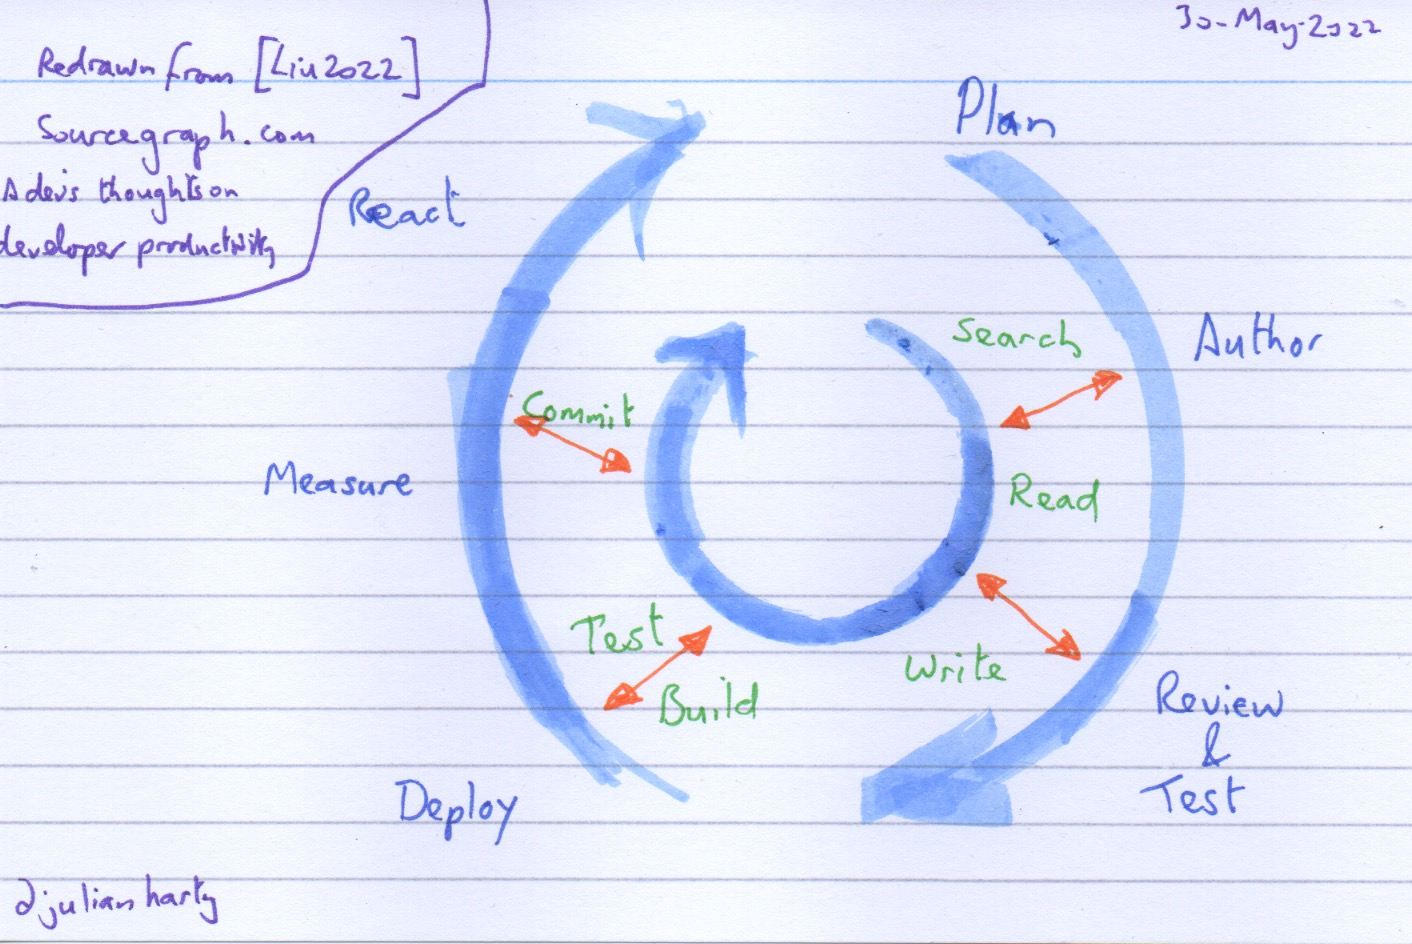
\includegraphics[width=12cm]{images/rough-sketches/developer-inner-loop-outer-loop.jpeg}
    \caption{Developer Inner Loop, Outer Loop\\ redrawn from \citep{liu2022_a_devs_thoughts_onDeveloper_productivity}}
    \label{fig:developer-inner-loop-outer-loop}
\end{figure}

\subsection{An iterative development lifecycle for app developers}
The research includes many findings that illustrate a conceptual iterative loop for app developers in terms of how their code is performing; to answer how's it doing in the real world. Figure \ref{fig:dev-app-reliability-iterative-loop} approximates various potential activities within this loop.

\begin{figure}
    \centering
    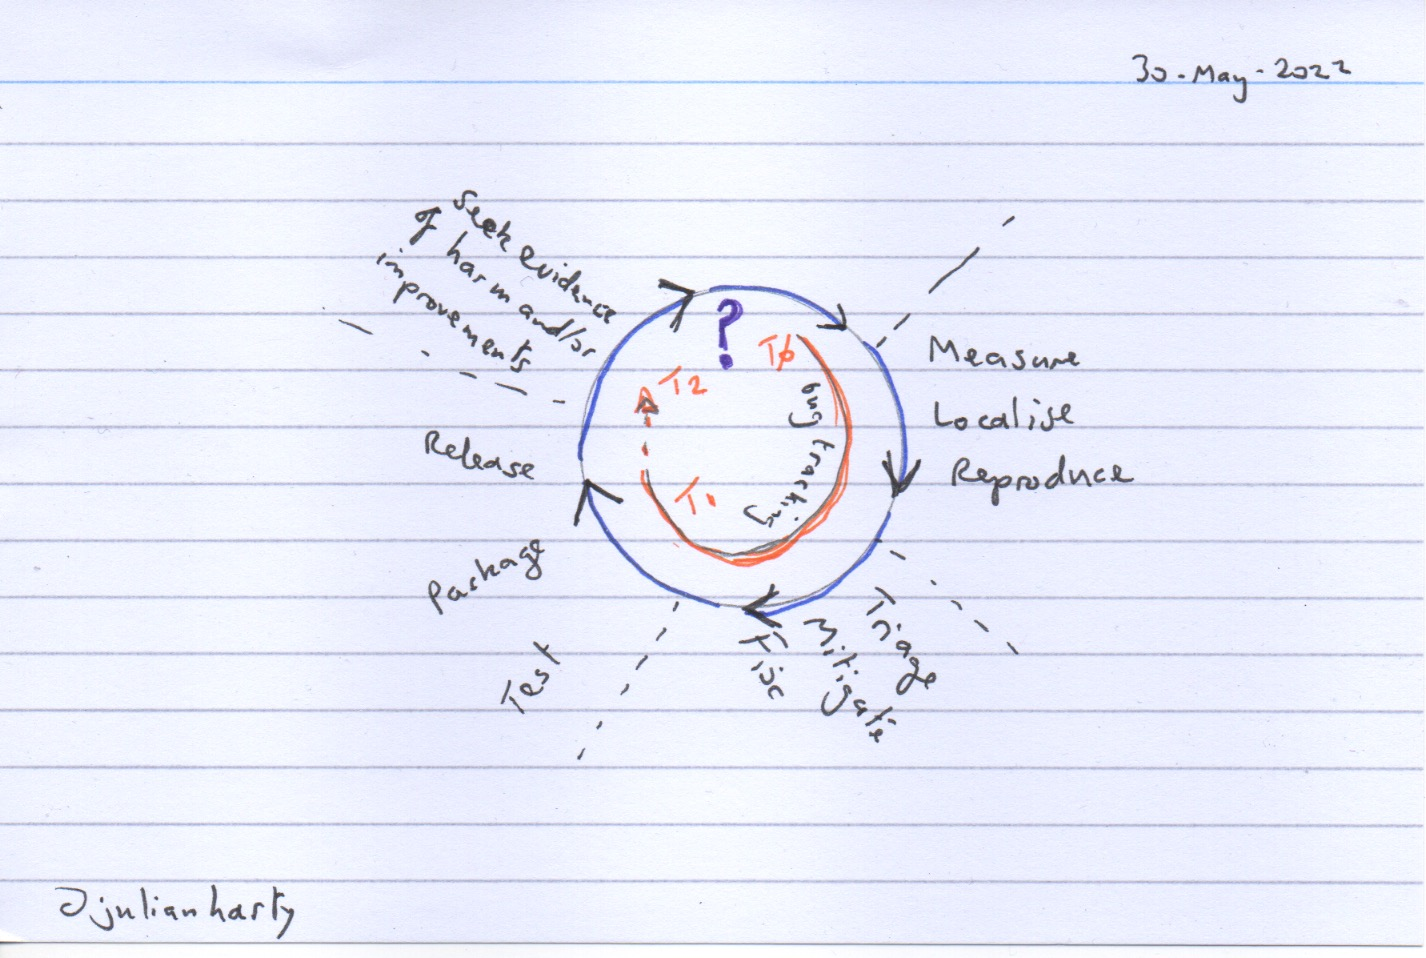
\includegraphics[width=12cm]{images/rough-sketches/dev-app-reliability-iterative-loop.jpeg}
    \caption{Developer's conceptual app reliability iterative loop}
    \label{fig:dev-app-reliability-iterative-loop}
\end{figure}

The loop starts with at the question-mark where the developers have a question about a flaw in the field related to their app's performance. They search for information which may include bug-localisation, adding logging to the app, and trying to reproduce the flaw using various techniques. They \emph{may} record the flaw in their issue tracking system, if so T0 marks the start of that bug in the bug tracking system.

They \emph{may} triage, mitigate, and/or attempt to fix the flaw, and if so they are likely to test the potential improvement(s), package the changes in a potential release and release it via the app store. Once the new release starts to be deployed they can start to seek evidence for any new/additional harm and/or any improvements in the performance of the app.

If the developer recorded the bug in the reporting system there are two more potential points of transition; T1 is when the developer believes the issue has been addressed for instance through modifications to the source code of the app, and T2 would be if there is evidence from the mobile analytics that the changes had the desired results. \emph{Not all teams/developers seek or record T2}.


\subsection{Sources of `truth'}\pending{This probably belongs in the Methodology}
In terms of the app and the artefacts there are several sources of `truth' in terms of the use of mobile analytics. These include:
\begin{itemize}
    \itemsep0em
    \item The developers: including what they say they do, and how they used mobile analytics.
    \item The source code, including the build scripts and relevant configuration files. The source code + the build process generates one or more application binaries, and they may also generate and run various automated tests that exercise the app and/or the mobile analytics SDK(s).
    \item The app binary: encapsulates and packages the software that is intended to run on end-user devices. 
\end{itemize}

This research included interviewing some app developers and working with others to learn about their perceptions of using mobile analytics and the artefacts they created in the process.

Whenever the source code was available it was studied to learn how mobile analytics had a) been integrated b) been used to effect changes in the source code. 

Binary analysis from the Exodus Privacy project was used to analyse the app binaries for the apps in the app-centric case studies.

\section{Summary of apps and their artefacts}
TBC




\noindent\textcolor[RGB]{220,220,220}{\rule{\linewidth}{1pt}}
\emph{older material follows and needs integrating.}

\noindent\textcolor[RGB]{220,220,220}{\rule{\linewidth}{1pt}}


\section{Normal and acceptable ranges of failures}
For the GTAF case study, the crash rates, as measured by Android Vitals, vary massively by release of the app (Al Quran (Tafsir \& by Word).\pending{A great deal more analysis is possible given the number of active apps and the ongoing access to Google Play Console.} 

Android Vitals does not report any failures in the GTAF taskinator app, which is created using React Native according to the development team. This is pertinent as similar behaviours in Android Vitals were observed for another app-centric case study, LocalHalo. 

